% !TEX root = main.tex

\section{句法分析}
句法分析是NLP中基础性工作,其分析句子的\textbf{句法结构}(主谓宾)和词汇间的\textbf{依存关系}(并列、从属),是语义分析、情感倾向、观点抽取等应用的基础。

\subsection{上下文无关法}
上下文无关法(Context-Free Gramma, CFG)由一系列规则组成,每条规则给出语言中某些符号可以被组织或排列在一起的方式。
\begin{figure}[H]
\centering
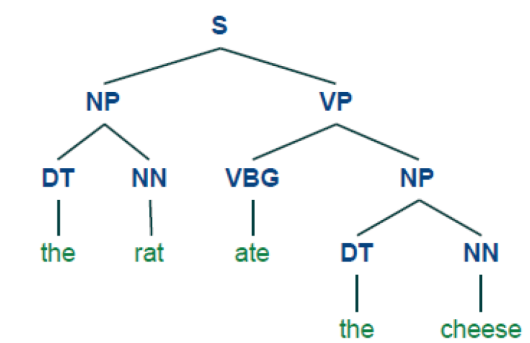
\includegraphics[width=0.4\linewidth]{fig/CFG.png}
\end{figure}
比如上述第一条规则为$S\to NP+VP$,然后$NP\to DT+NN$,一直到叶子结点的单词为止。

自底向上的线图分析法(chart parsing)\footnote{\url{http://www.inf.ed.ac.uk/teaching/courses/icl/lectures/2006/earley-lec.pdf}}:
\begin{itemize}
	\item 给定一组CFG规则:XP$\to\alpha_1\cdots\alpha_n,n\geq 1$
	\item 给定一个句子的词性序列:$S=W_1W_2\cdots W_n$
	\item 构造一个线图:一组结点和边的集合
	\begin{center}
	\begin{tikzcd}
	0\arrow[r]{W_1}\arrow[red,bend right,rr] & 1\arrow[r]{W_2}\arrow[red,bend left,rr] & 2\arrow[r]{W_3} & 3
	\end{tikzcd}
	\end{center}
	执行过程:查看任意相邻几条边上的词性串是否与某条规则的右部相同,若相同,则添加一条新的边跨越原来相应的边,新增加边上的标记为这条规则的头(左部)。
	重复这个过程,直到没有新的边产生。
\end{itemize}
\begin{figure}[H]
\centering
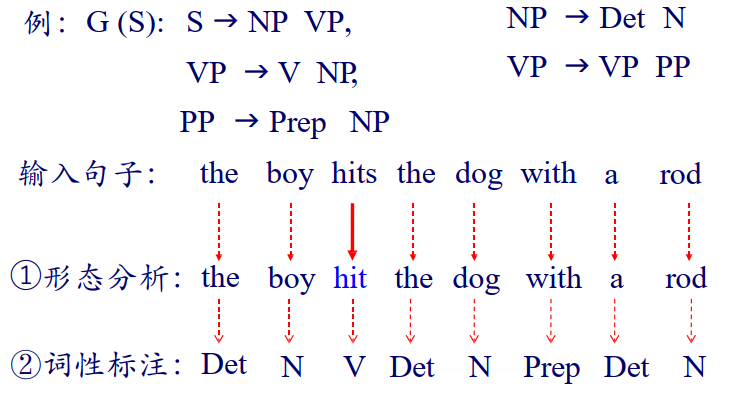
\includegraphics[width=0.6\linewidth]{fig/chart_parsing.png}
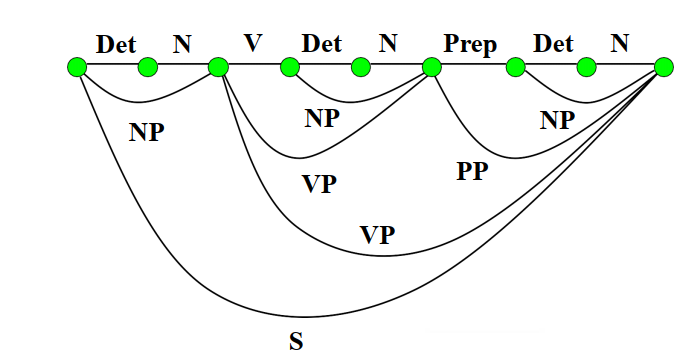
\includegraphics[width=0.6\linewidth]{fig/chart_parsing_2.png}
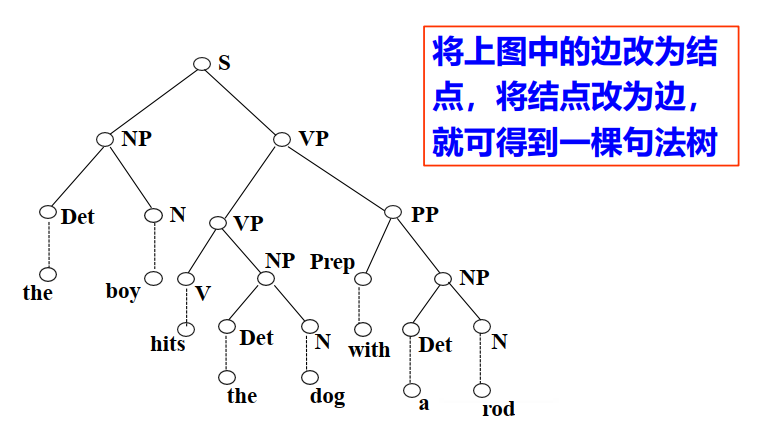
\includegraphics[width=0.6\linewidth]{fig/chart_parsing_3.png}
\end{figure}

CFG赋予语言层次化结构,但是根据CFG构建的语法分析树通常不止一个。

\subsection{概率上下文无关法}
为了应对产生多种语法分析结果的问题,引入概率上下文无关文法(PCFG):为每棵树计算一个概率。

PCFG规则
\[\begin{aligned}
&\text{形式:}A\to\alpha\qquad [p]\\
&\text{约束:}\sum_\alpha p(A\to\alpha)=1
\end{aligned}\]
如
\begin{flushleft}
NP $\to$ DT NN [$p=0.45$]\\
NN $\to$ leprechaun [$p=0.0001$]
\end{flushleft}

对于给定的语法分析树,可以计算其概率
\[P(T)=\prod_{i=1}^nP(RHS_i\mid LHS_i)\]
\begin{figure}[H]
\centering
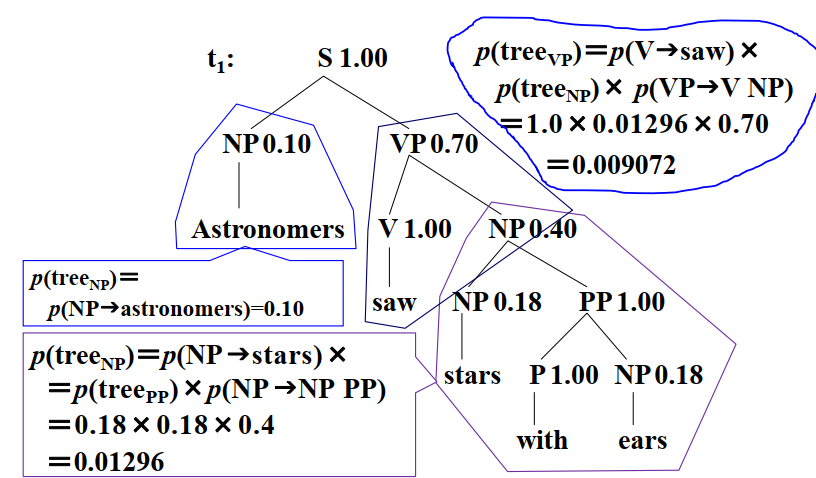
\includegraphics[width=0.6\linewidth]{fig/PCFG.png}
\end{figure}

\subsection{依存句法分析}
\begin{definition}[依存]
依存是指词与词之间支配与被支配的关系,这种关系是不对等的,有方向的。
处于支配地位的为支配者(governor),被支配地位的为从属者(modifier)。
\end{definition}
\begin{figure}[H]
\centering
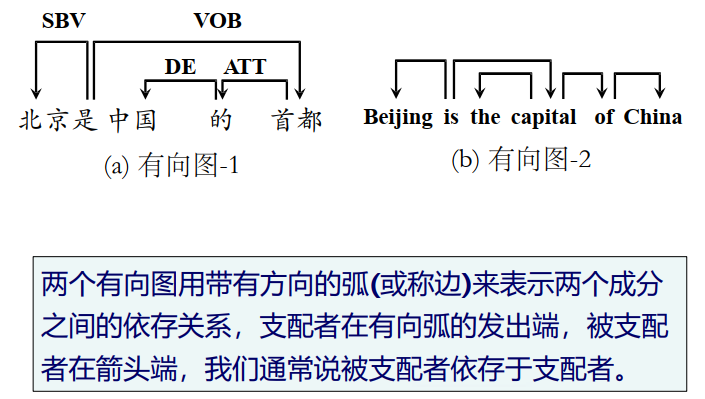
\includegraphics[width=0.6\linewidth]{fig/dependency_parser.png}
\end{figure}

依存语法的优势:
\begin{itemize}
	\item 依存关系和实际的语义关系比较接近,有助于对句子的语义方面的理解
	\item 定义相对比较简单,有助于高效率的句法分析
	\item 能够有效建模\textbf{长距离依赖关系},依存句法更适合词序列比较自由、灵活的语言
\end{itemize}

对依存图和依存树有约束:
\begin{itemize}
\item 一个句子只有一个独立的成分
\item 句子的其他成分都从属于某一成分
\item 任何一成分都不能依存于两个或多个成分
\item 如果成分$A$直接从属于成分$B$,而成分$C$在句子中位于$A$和$B$之间,那么,成分$C$或者从属于$A$,或者从属于$B$,或者从属于$A$和$B$之间的某一成分。
\end{itemize}
对应着对依存图和依存树的形式约束:单一父节点、连通、无环、可投射,由此来保证句子的依存分析结果是一棵有根的树结构。
\begin{figure}[H]
\centering
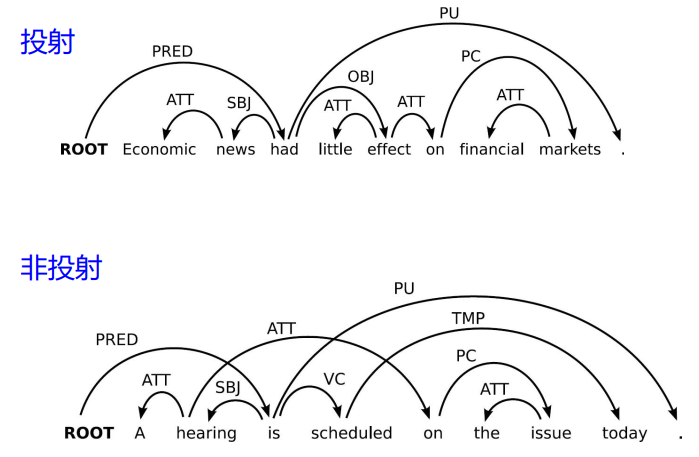
\includegraphics[width=0.6\linewidth]{fig/projective.png}
\end{figure}

依存结构表达的信息和短语结构句法树不一样,可以表达更长距离的信息依存关系。
\begin{figure}[H]
\centering
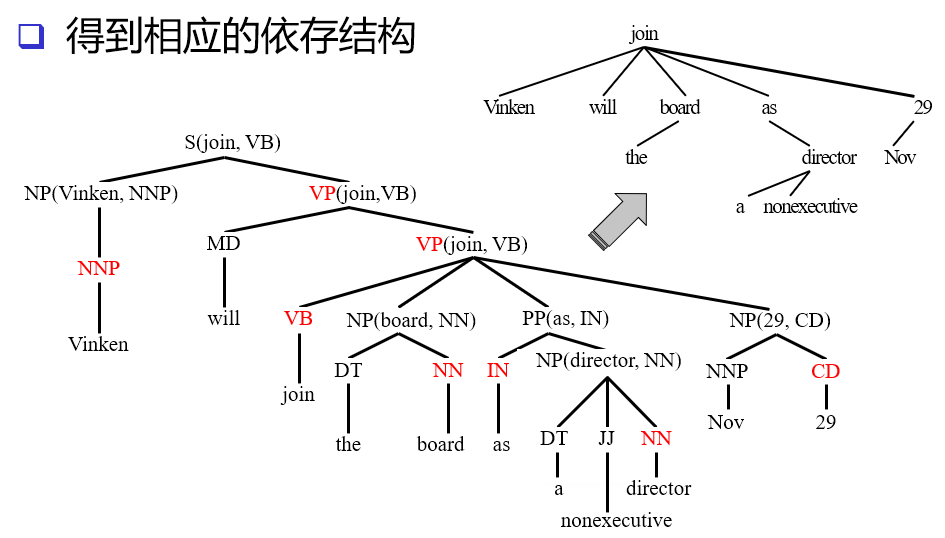
\includegraphics[width=0.6\linewidth]{fig/dependency_tree.png}
\end{figure}

短语结构可以转成依存结构:
\begin{itemize}
	\item 定义中心词抽取规则,产生中心词表
	\item 根据中心词表,为每个节点选择中心子节点
	\item 将非中心子节点的中心词依存到中心子节点的中心词上,得到相应依存结构
\end{itemize}